\section{First Exercise}
\subsection*{(a)}
\paragraph{Solution:} We know that 
\begin{equation}
    \left.\frac{\partial M(A,Z)}{\partial Z} \right|_A = 0
\end{equation}
for the minimum mass and from the lecture notes this gives 
\begin{equation}
    Z_\text{min}(A) \approx \frac{A}{1.98 + 0.015 A^{2/3}}.
\end{equation}
We now want to find for which $A$ we have $Z_\text{min} (A) = 28$ and $N = \text{even}$, where $N$ is the number of neutrons. Using the code found in App. \ref{app:1a}, the most stable nickel nuclide is $\nuc{Ni}{62}{}$.
\paragraph{Answer:} The most stable nickel nuclide is $\nuc{Ni}{62}{}$.

\subsection*{(b)}
\paragraph{Solution:} From the lecture it is known that the neutron drip line appears at
\begin{equation}
    S_\text{n} = B(A,Z) - B(A-1,Z) = 0
\end{equation}
and the proton drip line appears at
\begin{equation}
    S_\text{p} = B(A,Z) - B(A-1,Z-1) = 0,
\end{equation}
where $B(A,Z)$ is the binding energy which can be calculated from the Weizsäcker mass formula where it is given as
\begin{equation}
    B(A,Z) = a_\text{v} A - a_\text{s} A^{2/3} - a_\text{c} \frac{Z^2}{A^{1/3}} - a_\text{ass} \frac{(N - Z)^2}{A} + a_\text{p} A^{-1/2},   
\end{equation}
where $N = A - Z$ and the values for the constants are $a_\text{v} = \SI{15.9}{\mev}$, $a_\text{s} = \SI{18.4}{\mev}$, $a_\text{c} = \SI{0.71}{\mev}$, $a_\text{ass} = \SI{23.2}{\mev}$, and $a_\text{p} = \SI{11.5}{\mev}$. Implementing these equations in Python gives that the neutron drip line appears at $\nuc{Ni}{88}{}$ while the proton drip line appears at $\nuc{Ni}{52}{}$. The code can be seen in App. \ref{app:1b}. For fun, the code was run for $Z \in [4, 80]$ and the result was plotted against the nuclide chart. Both analyzing the actual chart as well as looking at Fig. \ref{fig:driplines} the calculation seems to give a bit too high of an $A$, but is reasonably accurate.

\paragraph{Answer:} The even-even Nickel nuclide that denotes the neutron drip line is $\nuc{Ni}{88}{}$ and the proton drip line is $\nuc{Ni}{52}{}$

\begin{figure}[t]
    \centering
    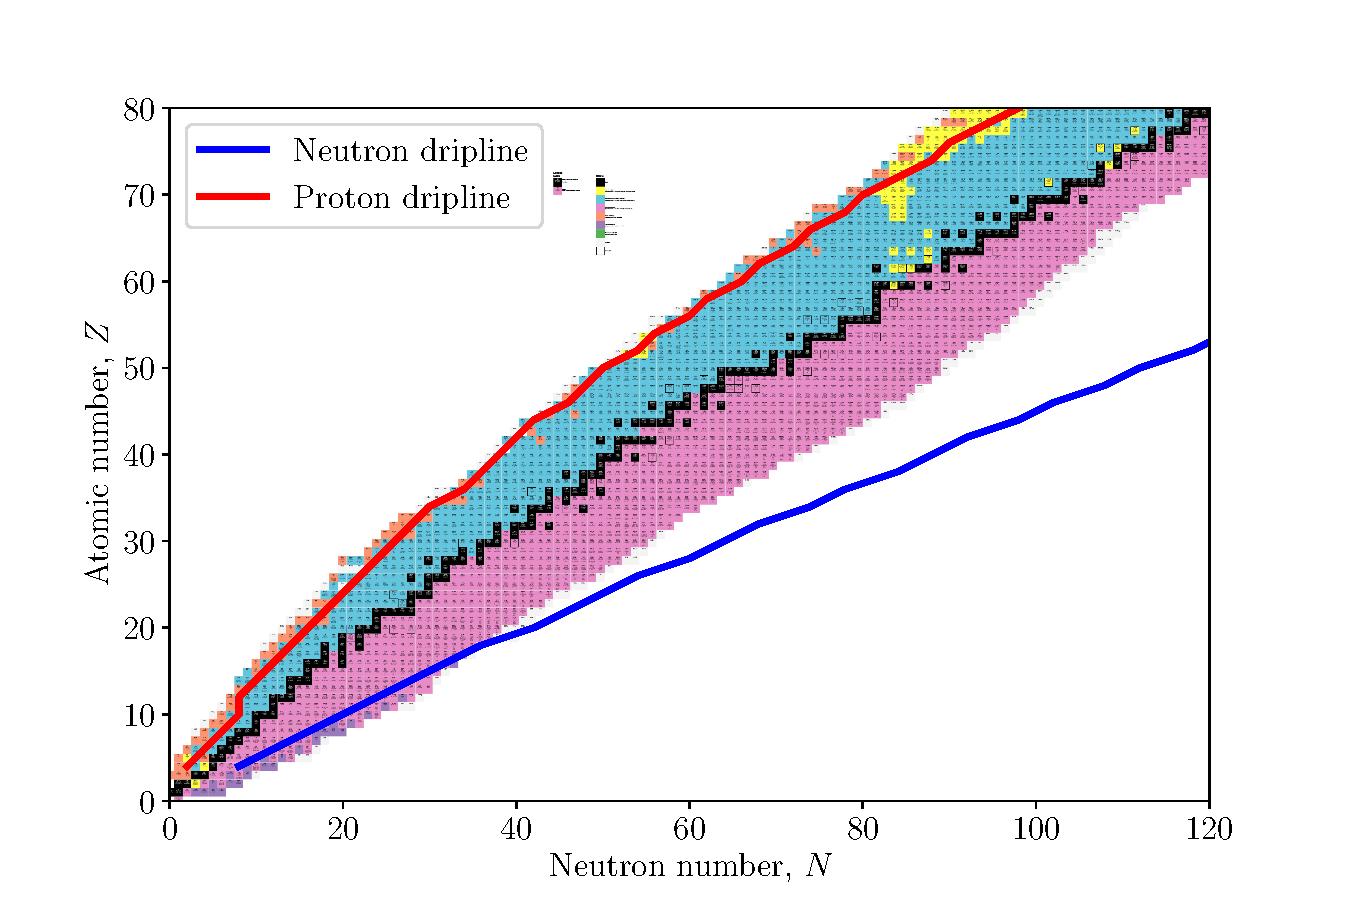
\includegraphics[width=\textwidth]{figures/driplines.pdf}
    \caption{The neutron and proton drip lines plotted for $Z \in [4, 80]$}
    \label{fig:driplines}
\end{figure}